\subsection{Laufzeitsicht}

In dem hier folgenden Kapitel soll dargestellt werden, welche Aktionen das System ausführt, um seine Funktionen bereitzustellen.
Dies erlaubt es, einen anderen Blickwinkel und damit ein besseres Verständnis für diese Anwendung zu erlangen.

Zu diesem Zweck wurden drei konkrete Abläufe ausgewählt.

\subsubsection{Anlegen eines neuen Agenten}

Der erste hier aufgeführte Fall soll beschreiben, welche Aktionen durchgeführt werden, um einen neuen Agenten anzulegen.

\begin{figure}[htb]
    \centering
    \includegraphics[scale=.65,center]{plant-diagrams/agent-creation-client-start.pdf}
    \caption{Client seitige Aktionen zum Anlegen eines Agenten}
    \ownsource
    \label{fig:agent-creation-client-start}
\end{figure}

Dabei beginnt der Ablauf mit dem Nutzer, der die Dateien auswählt, die seinen Agenten umfassen.
Die Dateien, die der Nutzer bereitstellt, sollen im Format eines npm-Paketes\footnote{\url{https://docs.npmjs.com/about-packages-and-modules}} sein.
Dies meint konkret, dass es im Wurzelverzeichnis eine package.json-Datei gibt, die neben der Version, dem Namen und der Beschreibung auch den Pfad zur Einstiegsdatei definiert.
Die dadurch festgelegte Einstiegsdatei ist der zweite erforderliche Bestandteil und muss eine kleine, aber zwingend erforderliche API implementieren.
Näheres dazu folgt in Kapitel \refsec{sec:artefacts}.

Zusätzlich kann er durch die package.json-Datei auch noch externe Abhängigkeiten definieren, die der Agent benötigt.
Diese werden dann bei der Installation mit installiert.

Alle bereitgestellten Dateien werden in Schritt \textbf{2.1} dann als Nachricht gebündelt.
Im Anschluss wird diese Nachricht dann an den Server gesendet.

\begin{figure}[tbp]
    \centering
    \includegraphics[scale=.65,center]{plant-diagrams/agent-creation-server.pdf}
    \caption{Der Server prüft den Agenten }
    \ownsource
    \label{fig:agent-creation-server}
\end{figure}

%\FloatBarrier

Dabei beginnt dieser mit der Prüfung der Daten und der Struktur in Schritt \textbf{3.1}.
In diesem Schritt wird vor allem sichergestellt, dass alle Informationen vorhanden und korrekt sind.
So wird beispielweise sichergestellt, dass der Name eine Mindestlänge hat und die angegebene Einstiegsdatei vorhanden ist.

Im Anschluss wird das Paket installiert.

Dafür werden im Zuge von Schritt \textbf{3.2} die mitgelieferten Dateien im Dateisystem abgelegt.
Dies ist notwendig, weil der ECMAScript-Standard in diesem Kontext keine synthetischen (in memory) Imports erlaubt und somit diese Dateien nur als ES Modules geladen werden können, wenn sie als Dateien vorhanden sind.

Idealerweise könnte man hier in der Zukunft einen, für diesen Zweck angepassten, ES Module Loader schreiben, welcher die Datei Inhalte im Arbeitsspeicher hält und diese direkt aus diesem laden kann.

Nach dem Schreiben ins Dateisystem wird er via Yarn im Schritt \textbf{3.3} installiert.
Damit sind dann seine Abhängigkeiten vorhanden und andere Pakete, wie der Agent Loader, können ihn referenzieren.

Hiernach wird versucht, den Agenten zu laden.

Dabei wird erst im Schritt \textbf{3.4} durch den Agent Loader eine Test-Sandbox (als Worker) mit dem Prüfscript geladen.
Diese erhält in \textbf{3.5} als Parameter die für den zu testenden Agenten vergebene ID.

%\FloatBarrier

Die Sandbox verhindert, dass der Server durch geladene Scripte oder durch Syntaxfehler leicht zum Absturz gebracht werden kann, und isoliert zusätzlich Fehlerquellen.

Durch das Installieren des Paketes kann dies hier nun durch die Namensreferenz aufgelöst werden und die Einstiegsdatei lässt sich durch einen asynchronen ES-Module import laden.

Durch das Laden prüft die Runtime implizit, ob der JavaScript-Code Syntaxfehler beinhaltet und ob alle Abhängigkeiten vorhanden sind.
Ebenso wird dadurch jeglicher Code ausgeführt, der nicht als Funktion verpackt worden ist.

Anschließend wird, falls das erfolgreich ist, im Schritt \textbf{3.11} geprüft, ob der Agent die notwendigen API Exports aufweist.
Dies soll vor allem dabei helfen, schnell strukturelle Fehler aufzudecken.

Sollte es hierbei zu Problemen gekommen sein, wird eine entsprechende Fehlermeldung generiert und an den Server bzw.
den Agent Loader zurückgegeben.

Im Diagramm wird der positive Fall dargestellt und das Erstellen eines Agenten ist somit mit \textbf{4.1} abgeschlossen.
In einem Fehlerfall würden nach \textbf{3.9} noch die umgekehrten Schritte bezüglich \textbf{3.2} und \textbf{3.3} folgen.

\begin{figure}[htb]
    \centering
    \includegraphics[scale=.65,center]{plant-diagrams/agent-creation-client-end.pdf}
    \caption{Der Client erhält die Antwort und stellt diese dar}
    \ownsource
    \label{fig:agent-creation-client-end}
\end{figure}

Durch den Socket wird dann die Rückmeldung an den Client gesendet.
Diese stellt der Client dann für den Nutzer dar.
In dem Diagramm \refgoal{fig:agent-creation-client-end} ist der positive Fall dargestellt.

Hierbei ist es wichtig, dass der Client durch diese Rückmeldung ebenfalls die Übersicht über die Agenten erweitert und dem Nutzer so darstellt, dass das Anlegen erfolgreich war.

\subsubsection{Erzeugung einer Instanz}

Als zweiten Anwendungsfall soll dargestellt werden, wie eine Instanz erzeugt wird, da dieser Ablauf zusätzlich hilft, ein besseres Verständnis hinsichtlich der Funktionsweise der Anwendung zu erlangen.

Das Erzeugen einer Simulationsinstanz besteht im Kern aus drei Abschnitten, bei denen vor allem Abschnitt eins uns drei nahezu identisch zu denen aus dem vorangegangenen Ablauf sind und deshalb hier nicht noch einmal wiederholt werden sollen, sondern nur kurz beschrieben werden.

Abschnitt eins beinhaltet auch hier die Nutzerinteraktion, bei der dieser das Straßennetz und den Agenten auswählt.
Zusätzlich vergibt er auch hier einen Namen und optional eine Beschreibung.
Der Client erzeugt dann daraus eine Nachricht, serialisiert diese und sendet sie an den Server.

Abschnitt drei verhält sich ebenfalls ähnlich und stellt das Erzeugungsresultat dem Nutzer dar.

Der zweite Abschnitt unterscheidet sich jedoch und beinhaltet die eigentliche Aktion des Systems, wie in dem folgenden Diagramm gezeigt werden soll.

\begin{figure}[htb!]
    \centering
    \includegraphics[scale=.65,center]{plant-diagrams/create-sim-main.pdf}
    \caption{Erstellung Simulationsinstanz, Server Thread}
    \ownsource
    \label{fig:create-sim-main}
\end{figure}

%\FloatBarrier

Beginnend mit dem Erhalt der Nachricht, fängt der Server an, die Aufforderung zur Erzeugung zu verarbeiten.
Um diese zu beantworten, beginnt der Server damit eine Liste aller Agenten und dann aller verfügbaren Layouts zu erzeugen.

Danach prüft er, ob er die IDs für das Layout und den Agenten in diesen Listen findet.
Sollte das der Fall sein, erzeugt er eine Simulation Instance, die in diesem Fall einen Realtime Handler hat.

Dieser Handler beinhaltet in seinem Konstruktor die Anweisung, einen neuen Node.js Worker zu erzeugen.
Sobald dieser erzeugt worden ist, wird eine Nachricht gesendet, die diesen Einstiegspunkt anweist, die eigentliche Instanz zu erstellen.

Schritt \textbf{4.1} ist also nur für die Node.js Worker verantwortlich und \textbf{4.2} beinhaltet die notwendigen Informationen für die eigentliche Simulationsinstanz.

Darunter befindet sich vor allem die Konfiguration des Agent Loaders, die ID des Agenten und das initiale Layout, das nicht als ID, sondern als World Objekt übertragen wird.

Auch diese Nachricht wird, wie auch die Nachrichten, die an den Client gesendet werden, mit den gleichen Werkzeugen serialisiert.
Dies wird hier zur Übersichtlichkeit nicht gezeigt, ist aber für die Anwendung relevant, um die notwendige Geschwindigkeit aufrechtzuerhalten.

Danach beginnt der Instance Main Connector mit der Verarbeitung, was in der folgenden Abbildung dargestellt werden soll.

\begin{figure}[htb]
    \centering
    \includegraphics[scale=.65,center]{plant-diagrams/create-sim-worker.pdf}
    \caption{Erstellung Simulationsinstanz, Worker Thread}
    \ownsource
    \label{fig:create-sim-worker}
\end{figure}

%\FloatBarrier

Hierbei wird der Instance Main Connector durch die Erzeugung des Workers automatisch instanziiert.
Im Anschluss wartet dieser auf das Instanzerzeugungs-Kommando, das die oben genannten Informationen enthält.

Durch diese kann er dann den Agent Loader erzeugen und mit diesem dann den Agenten anhand seiner ID laden.

Im Anschluss wird aus den Informationen, die übertragen worden sind, eine Welt erzeugt.
Diese Erstellung inkludiert vor allem die Instanziierung der Klassen, denn die übertragenen Objekte haben keine Assoziationen mehr mit diesen.

Danach wird in Schritt \textbf{5.7} die tatsächliche Simulations-Instanz erzeugt.
Sie steuert den Agenten an und verwaltet den Weltzustand.

Durch sie kann später ein neuer Frame angefragt werden.
Die Instance Main Connector Klasse so wie die Simulation Instance Realtime Handler Klasse könnte beide vernachlässigt werden und die Simulation Instance könnte direkt von dem Server angesprochen werden, sollte man keine Isolation oder Multithreading verwenden wollen.

Sollte diese Erzeugung funktioniert haben, dann meldet der Instance Main Connector nun den Ready Status zurück.
Daraufhin trägt der Server diese Instanz in seinem Register ein und meldet die neue ID der Instanz an den Client zurück.

In diesem Zustand könnten nun Frames von dem Handler bzw. der Simulation Instance angefragt werden.

\FloatBarrier

\subsubsection{Der Frame-Passthrough}

\newcommand{\processbegin}[2]{\item[$\mapsto$] \textbf{\textit{#1} #2:}}
\newcommand{\processstep}[2]{\item[$\rightarrow$] \textbf{\textit{#1} #2:}}

Der Frame-Passthrough umfasst alle Schritte, die notwendig sind, um durch das initiale Zeitgeber-Signal einen Pixel-Buffer zu füllen.

Für diesen sollen die übergreifenden Prozesse nur kurz textuell beschrieben und ausschließlich der Entitätsumformungsprozess im Detail beleuchtet werden.

Zentral zu beachten ist, dass der Prozess der Darstellung und der Berechnung der Frames bei dieser Anwendung voneinander getrennt sind und parallel zueinander laufen.
Verbunden sind diese Prozesse durch die Synchronisation des Zustandes der Welt sowie die zeitliche Synchronisation durch die Bildwiederholrate.

Somit muss unterschieden werden, welcher Prozess betrachtet wird.
Sie werden daher hier auch getrennt voneinander beschrieben.

Begonnen werden soll mit dem des Servers.
Dieser hat im Grunde einen sehr einfachen Zyklus, der hier Schritt für Schritt aufgelistet werden soll.

Jeder Stichpunkt repräsentiert einen Schritt und dieser ruft den nächsten auf bzw. leitet an ihn Daten weiter.

\textit{SR} = Backend Server Realm, \textit{WR} = Worker Simulation Instance Realm

\begin{itemize}
    \processbegin{SR}{Frame Loop 60 Hz Signal} Begonnen wird bei der Frameloop, die 60 Mal die Sekunde ein Signal sendet.

    \processstep{SR}{Simulation Instance Realtime Handler} Der Realtime Handler, der auch den Timer beinhaltet, woher auch sein Name stammt, nimmt dieses Signal auf und leitet es an seinen Worker weiter.
    Zusätzlich erneuert er interne Caches und benachrichtigt im Anschluss zu der Frameerzeugung alle Event Listener.

    \processstep{SR}{Simulation Instance Message Serializer} Diese Serialisierungs-Einheit formt die JavaScript-Werte und Objekte in ein Binärformat um, damit sie transferiert werden können.
    Dieser Schritt wäre nicht gezwungenermaßen notwendig, insofern der interne Serialisierer dies sonst machen würde, jedoch erlaubt dieser, die Werte direkt serialisiert weiter an den Client zu reichen und nicht im SR später erneut serialisieren zu müssen.

    \processstep{WR}{Simulation Instance Message Serializer} Dieser Serialisierer ist das entsprechende Gegenstück und wird vor allem zum Serialisieren der Frames benötigt.

    \processstep{WR}{Instance Main Connector} Die Komponente ist in dem Kontext der Verwendung des Workers geschrieben worden.
    Sie baut die Verbindung zu dem Server Thread auf und verwendet den Serialisierer.
    Nach der Instanziierung erwartet sie die Initialiserung-Nachricht und erlaubt im Anschluss das Anfragen neuer Frames.
    Sie schirmt den Verwendungskontext bezüglich der Simulation Instance ab.

    \processstep{WR}{Simulation Instance} Diese Komponente ist die Fassade für die eigentliche Simulation.
    Sie beinhaltet Methoden, die das Verwalten vereinfachen und erhält das durch den Instance Main Connector erhaltene Signal in Form von Aufrufen der \textit{calculateNextFrame} und \textit{getCurrentFrame} Methoden.

    \processstep{WR}{Simulation Engine} Die Simulation Instance hat das Ziel die Verwendung für den Client bzw.
    deren kumulierte Anfragen zu beantworten.
    Im Gegensatz dazu ist die Simulation Engine mehr low level und hat im Grunde nur Getter und Setter so wie die Frame Iterationslogik.
    Sie verwalten auch den Agenten und sie ist der beabsichtigte Weg diesen zu verwenden.

    \processstep{WR}{Agent} Der Agent ist die Instanz, die durch die Simulation Instance erzeugt worden ist.
    Der Agent wird durch den Konstruktor, der in den Agenten-Dateien definiert worden ist, erzeugt und erhält dabei Kontextinformationen sowie eine Referenz zu der Simulation Instance, die ihn erzeugt hat.
\end{itemize}

Ab dem Agenten lässt sich die Nachverfolgung des Frame Signals nicht fortführen, da sich die nach folgenden Schritte nicht generalisieren lassen.
Im Fall des Beispielagenten, der im Rahmen dieser Arbeit entwickelt worden ist, werden innerhalb des Agenten dann zuerst alle freien Spawn Plätze belegt und dann im Anschluss alle Fahrzeuge synchron, wenn möglich, bewegt.

Unabhängig von diesem internen Ablauf wird, wenn der Agent eine neue Welt zurückgeliefert hat, dieser Ablauf rückwärts ausgeführt.
Der Realtime Handler benachrichtigt dann alle eingetragenen Listener.
Diese stammen aus Clients, die über den aktuellen Zustand dieser speziellen Instanz benachrichtigt werden möchten.

Der Client als solcher läuft zu diesem Ablauf parallel.
Dieser hat dafür einen eigenen Zeitgeber, damit die Darstellung für den Nutzer flüssig bleibt.

Sollte ein Client registriert sein, erhält er durch den folgenden Ablauf den aktuellen Weltzustand.

\textit{SR} = Backend Server Realm, \textit{MR} = Frontend Main Realm, \textit{GT} = Graphics Thread

\begin{itemize}
    \processbegin{SR}{Instance Changed Event} Dies ist das Event, das durch die Rückmeldung vom Worker Thread zustande kam.

    \processstep{SR}{Simulation Instance Realtime Handler} Es wird vom Simulation Instance Realtime Handler angenommen und für Caches verarbeitet.
    Im Anschluss ruft dieser alle auf ihm registrierten Listener auf.

    \processstep{SR}{Individual WebSocket Handler} Dieser Handler hatte sich, durch die Client Nachricht cm-start-sending-frames bei der Simulations-Instanz für Veränderungen angemeldet.
    Er formt das Event nun um und sendet es weiter.
    Dabei muss der Frame nicht erneut serialisiert werden, da er noch serialisiert im Speicher liegt.
    Er kann bei allen WebSocket Handlern einfach in eine entsprechende Nachricht verpackt werden was enorm Ressourcen spart und den Server Thread responsiv hält.

    \processstep{SR}{Client-Server Partial Serialiser} Der Partial Serialiser, so genannt, weil er den Frame nicht serialisiert, serialisiert auch hier die Nachricht und sendet sie in einem minimal Binärformat an den Client über das WebSocket Protokoll.
    Dieses erlaubt einen bidirektionalen Nachrichtenaustausch und hilft somit bei der latenzarmen Frameübermittlung.

    \processstep{MR}{Client-Server Serialiser} Der Client Serialiser entpackt die Nachricht nun vollständig samt dem Frame und erzeugt wieder JavaScript Values.
    Diesen neuen Frame hängt er einer Redux Action an und dispatched diese auf dem Store.

    \processstep{MR}{Redux Store/Reducer} Der Store leitet diese dann weiter an den received-frame Reducer, der einen neuen Store-Zustand erzeugt, was wiederum alle Store-Subscriber benachrichtigt.

    \processstep{MR}{Simulation State Controller} Der State Controller ist die Einheit, die durch das React Element erzeugt wird und die übergeordnete Verbindung zwischen React, Redux und der Render-Pipeline herstellt.
    Er wird bei Frame-Änderung benachrichtigt und gibt den Frame an den Renderer weiter.
    Zusätzlich wird er auch in die Animation Loop eingebunden und erlaubt das Selektieren von Entitäten.

    \processstep{MR}{Render Pipeline Handler} Dies ist der Handler, der das eigentliche Rendering übernimmt.
    An ihn wird der Frame übergeben, den er speichert und dann die Frame dirty Flag setzt.
\end{itemize}

Nun sind der aktuelle Frame sowie alle weiteren notwendigen Informationen im Renderer hinterlegt.
Dieser hat, wie bereits angemerkt, seinen eigenen Zeitgeber, der von der Bildwiederholrate des Bildschirms so wie dem Betriebssystem abhängt.

Er wird durch den Browser in Form eines Events bereitgestellt.

\begin{itemize}
    \processbegin{MR}{Animation Frame Event} Dieses Event wird vom Browser erzeugt und an JavaScript weitergereicht. Es erlaubt eine Bildschirm abhängige Bildwiederholrate einzuhalten.

    \processstep{MR}{Show Simulation Controller \textit{(Clicks/Hover verarbeiten)}} Der Show Simulation Controller nimmt das Signal an und beginnt damit den Interaction Event Buffer zu verarbeiten und die Interaktionen auf die Entitäten anzuwenden.

    \processstep{MR}{Render Pipeline Handler \textit{(Weltzustand anwenden)}} In diesem Schritt nutzt der Handler den hinterlegten Frame und die Pipeline und wendet die Pipeline auf den Frame an.
    Dies ist der integrale Schritt, in dem aus den TRISS Entitäten der three.js\footnote{\url{https://threejs.org/}} (Teil-)Szenengraph erzeugt wird.
    Er ist ein sehr zeitintensiver Schritt, der für jeden Frame von dieser Anwendung ausgeführt werden muss.

    \processstep{MR}{Render Pipeline Handler \textit{(Resizing)}} Der Resizingschritt synchronisiert jeden Frame die Größe des Canvas, den Platz, der zur Verfügung steht, und die Seitenverhältnisse der three.js Kamera.

    \processstep{MR}{3D Rendering} In diesem Schritt werden die neuen Entitäten in den three.js Szenengraphen übergeben und three.js angewiesen, diese mit der hinterlegten Kamera auf den eingesetzten Canvas zu zeichnen.
    Er stößt bibliotheksinterne Prüfprozesse an und transferiert im Anschluss alle Informationen über den Graphen in GL\_Buffer Instanzen, die zum Informationsaustausch mit der GPU genutzt werden.

    \processstep{GT}{OpenGL Shader Ausführung} Im Anschluss wird der OpenGL Shader ausgeführt, der durch three.js erzeugt und verwaltet wird.
    Er erhält Informationen wie beispielsweise Matrix4 Arrays und Geometry Buffer der Szene und erzeugt daraus eine Pixel Array, die dann durch den Browser als Inhalt für die Canvas DOM Node verwendet wird womit dann repräsentative Pixel für die Szene durch die Anwendung dargestellt werden.

    \processstep{MR}{CSS Rendering} Ein weiterer Schritt ist es, three.js mit den gleichen Informationen wie für den 3D-Rendering-Schritt anzuweisen, die 2D-Elemente zu \enquote{rendern}.
    Dabei werden durch diesen Schritt nur die Elemente des Szenengraphs durch three.js verarbeitet, die von der CSS2DObject\footnote{\url{https://threejs.org/examples/\#css2d_label}} Klasse erben.
    Diese Elemente können dann auch im Szenen World Space (genauso wie Kacheln und Fahrzeuge) platziert werden.
    Die auf den View Space umgeformten Koordinaten werden dann auf ein HTML Wrapper angewendet, wodurch die Illusion entsteht, dass ein HTML Element im 3D platziert worden ist.
    Dies wird in dieser Anwendung für Metainformationen der Entitäten verwendet, die durch React erzeugte DOM Fragmente repräsentieren und durch three.js in respektive zur Kamera positioniert werden.

    \processstep{GT}{OpenGL DOM Rendering} Im Anschluss fügt der Browser den Buffer des Canvas und seine Positionierung zusammen und stellt ein Bild der Webseite bzw.
    der Anwendung dar.
\end{itemize}

Auch wenn der Server, angewiesen durch seinen eigenen Zeitgeber, mehr oder weniger Frames sendet als die Menge, die durch den Client potenziell verarbeitet werden kann, hat das keinen direkten Einfluss auf die Framerate des Clients.
Dies wird dadurch behandelt, dass die Pipeline, also der aufwendige Verarbeitungsprozess, nur dadurch angestoßen wird, wenn der Browser tatsächlich ein neues Bild benötigt.
Die Pipeline verwendet dafür immer den aktuellsten Zustand, den der Client erhalten hat.

Dieser wird im Schritt \textit{Weltzustand anwenden} von seiner übertragenen Form in eine Form umgewandelt, die an OpenGL übertragen werden kann.

Zwei dieser Abläufe sind dabei für die Funktionsweise dieser Anwendung integral.

Der erste ist, dass der von dem Agenten erzeugte Frame nach seiner ersten Serialisierung im WR nicht wieder komplett im SR deserialisiert wird, sondern dort nur neu verpackt wird.
Das erlaubt es dem SR, hier bedeutend Ressourcen zu sparen und responsiv für andere Kommandos bzw. Verbindungen zu bleiben.

Ebenso ermöglicht das ihn auch, ohne nennenswerten Mehraufwand, mehrere Clients mit dem gleichen Zustand einer Simulation zu beliefern, oder diesen abzuspeichern.

Der zweite relevante Aspekt ist die Umformungsoperation, die notwendig ist um aus den Positions- und Orientierungsinformationen, die der Server als Weltzustand liefert, Buffer und Meshes zu erzeugen, die durch die GPU in einen Pixel Buffer umgeformt werden können.

Dabei wurde bei der Entwicklung Inspiration von den Nodes\footnote{\url{https://docs.blender.org/manual/en/3.2/compositing/introduction.html}} \footnote{\url{
https://docs.blender.org/manual/en/3.2/render/shader_nodes/index.html}} der Blender Suite bezogen.

Diese stellen Funktionen und deren Aufrufe als Fluss von Daten dar, bei denen die Funktionen als Knoten in einem Graphen dargestellt werden und deren Eingabeobjekte auf der linken und die Ausgabe der Funktion auf der rechten Seite der Knoten angebracht sind.
Diese Darstellung erlaubt einen guten Überblick und impliziert eine gute Modularität sowie Erweiterbarkeit.

Nicht zuletzt stellt dieser Ansatz die Daten und deren Fluss durch Verarbeitungsschritte in den Vordergrund und priorisiert dadurch auch die Entwicklung anders.

Interessanterweise gibt es mittlerweile auch bei three.js die Bestrebung, einen Node Renderer zu erschaffen, der eine Alternative zu dem klassischen auf einem Szenengraphen basierenden 3D-Renderer darstellt.
Ein Beispiel seiner Verwendung kann in dem three.js example \enquote{node/playground}\footnote{\url{https://threejs.org/examples/?q=node\#webgl\_nodes\_playground}} gefunden werden.

Dieser soll jedoch primär Low-Level-Daten und -Strukturen verwalten und verwendet werden, um dynamisch Shader Programme zu erzeugen.
Dies ist in diesem Programm nicht der Fall, es wird hier nach wie vor der Szenengraph von three.js verwendet, die dafür notwendigen Entitäten werden allerdings via diesem Ansatz erzeugt.

Der durch die Stichpunkte beschriebene Ablauf ist der generelle Frame Passthrough.
Nun soll im Folgenden konkreter dargestellt werden welche Knoten bzw. Funktionen im Umformungsprozess von TRISS Entitäten zu three.js Entitäten Verwendung finden und welche Rolle sie spielen.

Exemplarisch sollen dafür die Knoten dienen, welche für die Darstellung der Kacheln einer laufenden Instanz benötigt werden.

Dieses Data-Flow-Diagram\footnote{\url{https://www.lucidchart.com/pages/data-flow-diagram}} ist dabei von links nach rechts zu lesen.
Die Nummerierungen der Aktionen definieren die Reihenfolge, wobei die Aktionen mit gleichem Ganzzahl-Anteil unabhängig voneinander stattfinden.

\begin{sidewaysfigure}[htbp]
    \centering
    \label{fig:render-pipeline-dfd}
    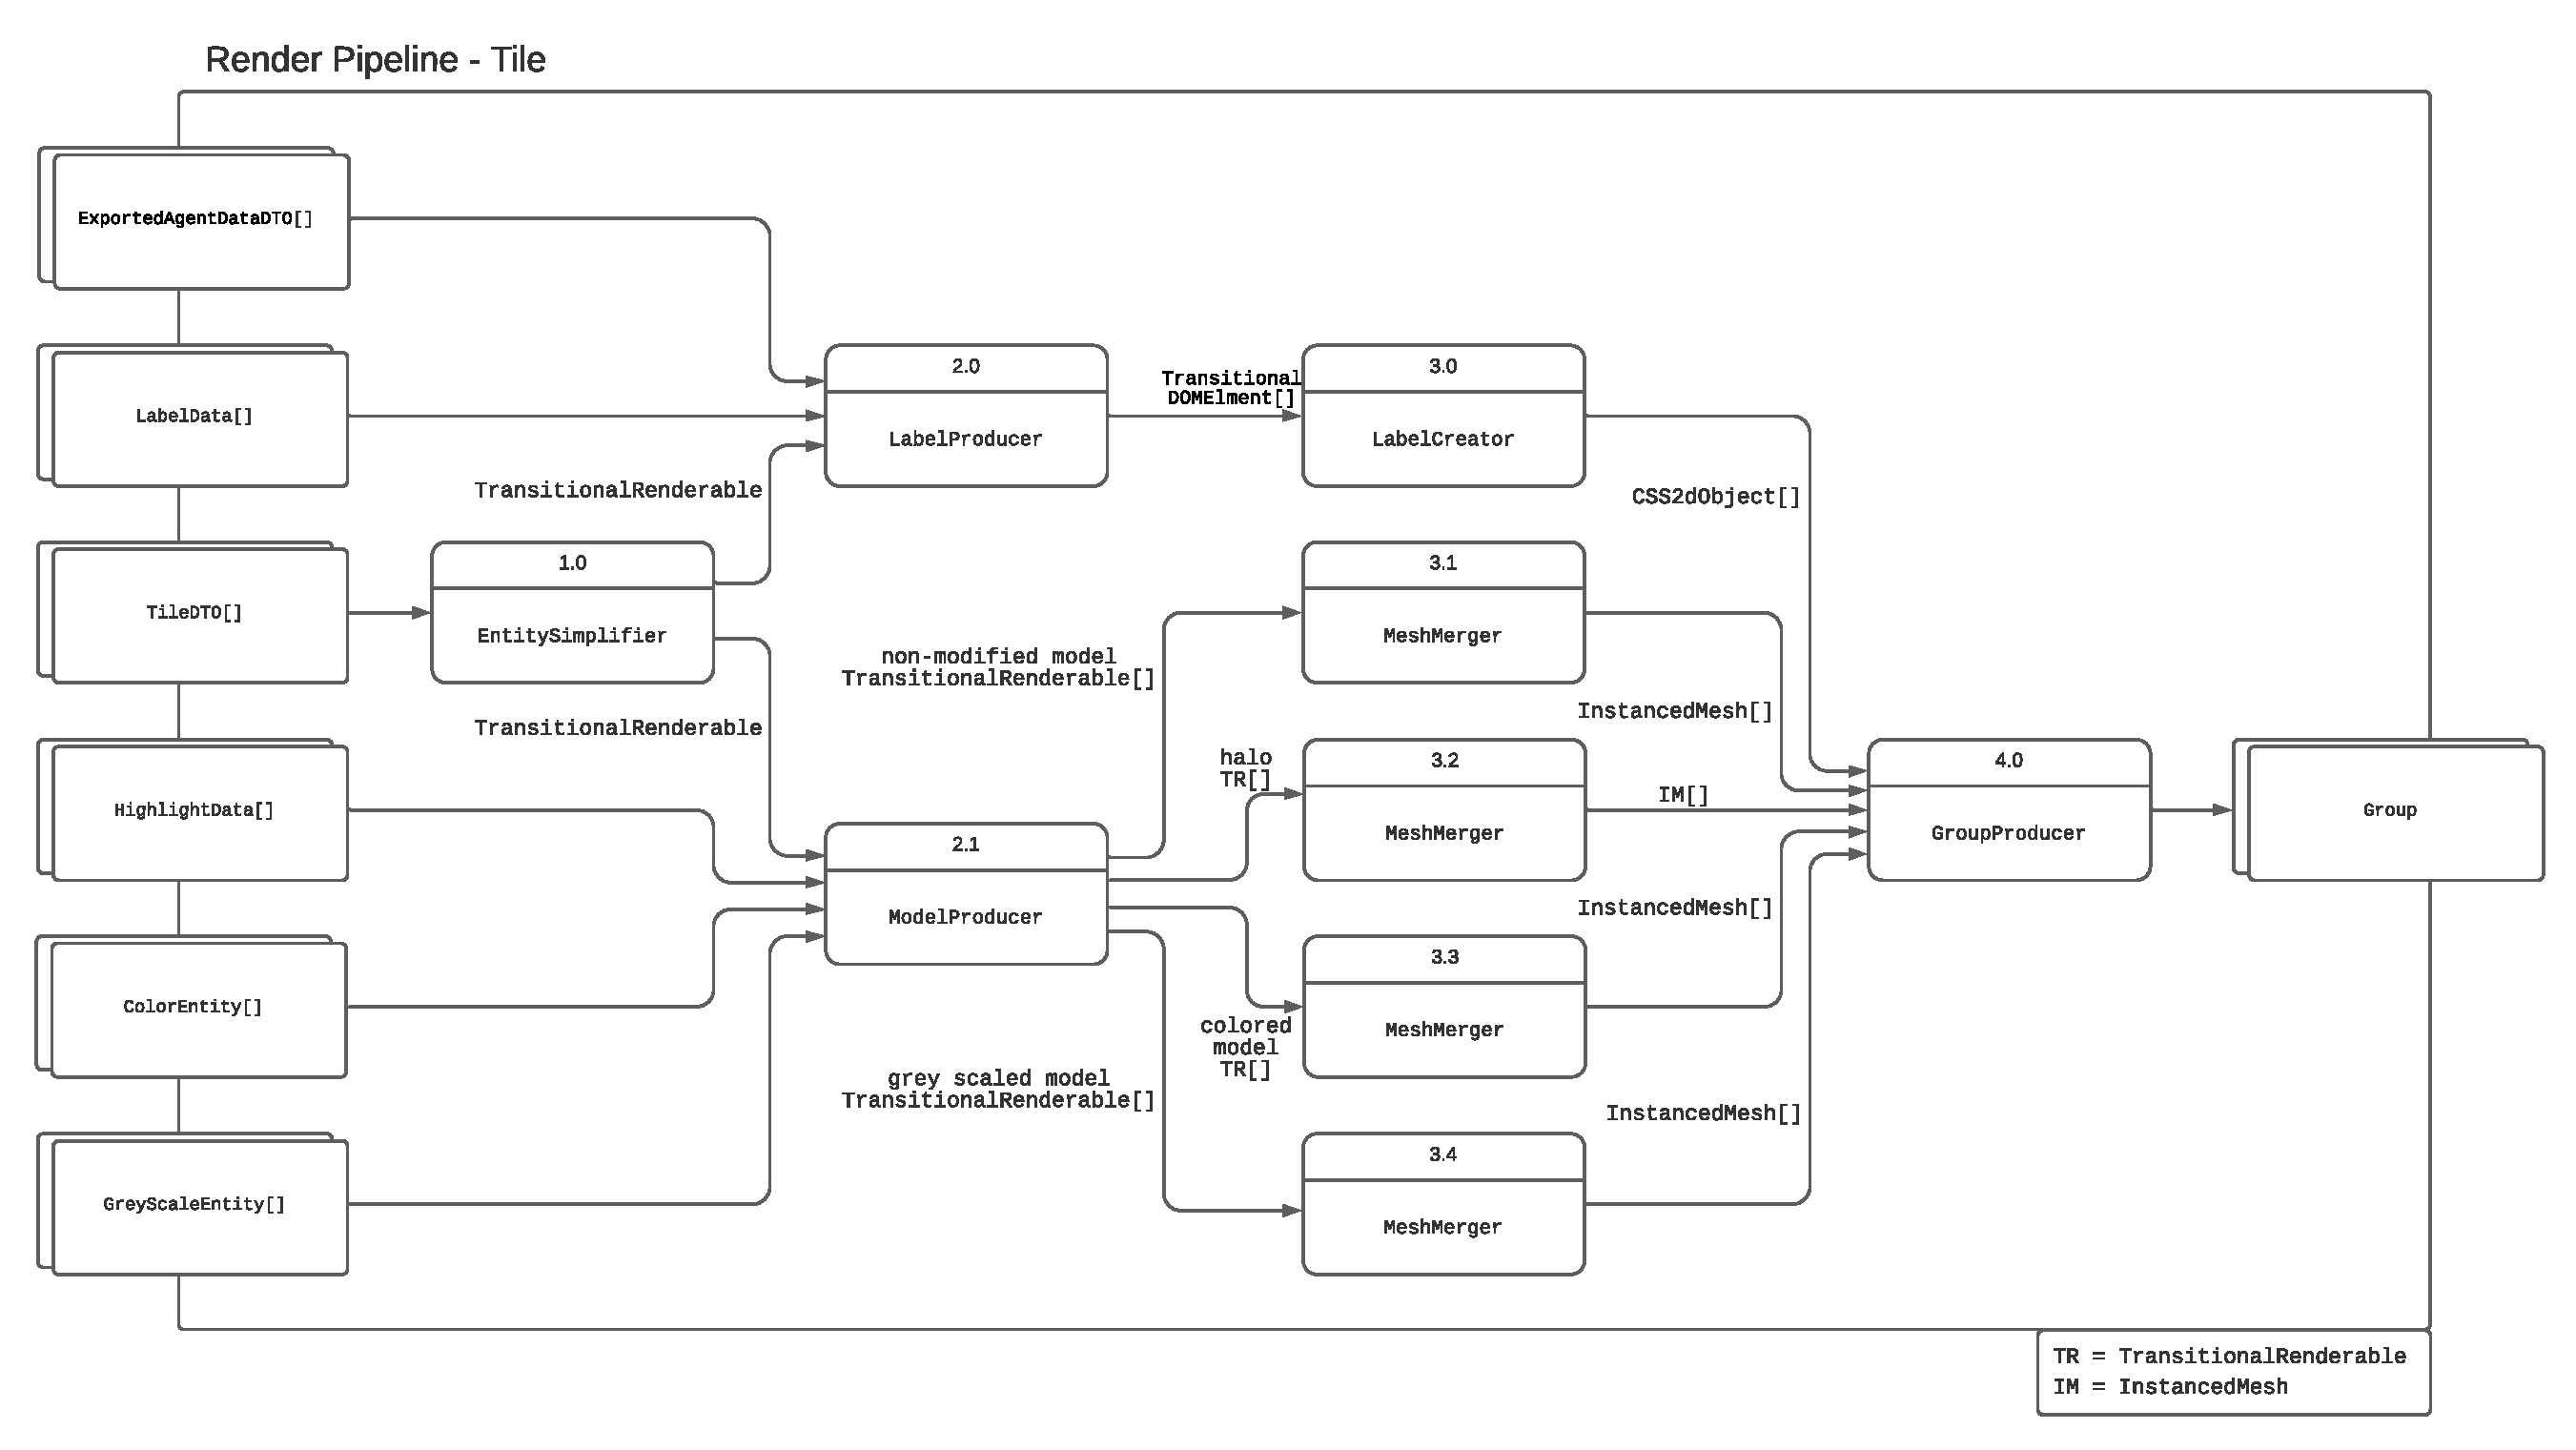
\includegraphics[scale=.65,center]{medien/render-pipeline-dfd.pdf}
    \caption{Render Pipeline: Tile DfD}
    \ownsource
\end{sidewaysfigure}

%\FloatBarrier

Das Diagramm zeigt alle Schritte, die nötig sind, um die Kacheln, die der Handler erzeugt hat bzw. bereitstellt, in solche umzuwandeln, die dem three.js Szenengraph hinzugefügt werden können.
Vom Server bzw. dem Agenten kommen die Entitäten Exported Agent Data DTO und Tile DTO.
Alle weiteren wurden vom Handler auf Grundlage der Nutzerinteraktionen erzeugt.
Beispielweise führt der Klick eines Nutzers zu einer Highlight Data Entität.
Die Grey Scale Entity wird wiederum verwendet, um eine Kachel bei der Platzierung anzudeuten.

Die Datentypen werden im Graphen dann durch den Text an den Kanten angedeutet, dabei wurde aus Lesbarkeitsgründen an einigen Stellen der Datentyp abgekürzt.
Über dem Datentyp wurde, dort wo es nicht eindeutig war, noch der semantische Typ mit angebracht.

Die Umwandlung startet bei der Vereinfachung der Entitäten, wobei aus der Grid Position die eigentlichen Weltkoordinaten errechnet werden.
Aus der Himmelsrichtung-Orientierung wird dann der Quaternion\footnote{\url{https://en.wikipedia.org/wiki/Quaternion}} errechnet.
Diese beiden erzeugen in diesem Schritt auch die 4x4 Matrix, die im weiteren Verlauf für die Positionierung des Modells gebraucht wird.

Besagtes Modell wird ebenfalls in diesem Schritt, durch den beigefügten Tile Type von einem globalen Service angefragt und dem Ausgabewert beigefügt.
Diese Grundlage verwenden dann die Schritte \textit{2.0} und \textit{2.1}.

Schritt \textit{2.0} verwendet dabei die zusätzlichen Eingabedaten, um React mit den entitätstatischen Wrappern und den Agent Data zu versorgen.
Dass der HTML-Wrapper statisch und mit der Entität verknüpft ist, ist wichtig, damit React in der Lage ist, inkrementelle Änderungen anzuwenden und den internen Zustand zu assoziieren, was enorme Ressourcen spart und Interaktivität ermöglicht.

Der Label Producer erzeugt dann ein Ausgabeobjekt, das in einem weiteren Schritt in ein CSS 2D Object umgewandelt wird, das von three.js verwendet werden kann und korrekt in Relation zum Canvas platziert wird.

Schritt \textit{2.1} ist noch einmal bedeutend aufwendiger und sorgt intern dafür, dass alle notwendigen Models und deren Abwandlungen erzeugt werden.
Dafür werden Kopien des Meshes erzeugt und mit neuen Materialien versehen.

Im Anschluss werden all diese Modelle mit ihren Matrizen an die jeweiligen Mesh Merger weiter geleitet.
Hierbei ist es wichtig, dass eine Instanzstabilität herrscht.
Das heißt, dass bei gleicher Eingabe nicht nur die gleiche Ausgabe erzeugt wird, sondern dass auch die Instanzen, die referenziert werden, stabil sind.
So wird bei jeder Tile \textit{34} (eine Gerade), die Grey Scaled werden soll, immer die gleiche 3D-Modell-Referenz zurückgegeben.

Dies und die Aufteilung in mehrere Mesh Merger ist sehr wichtig, damit effizient Instanced Meshes daraus gebildet werden können.
Die jeweiligen Mesh Merger erhalten vollständig getrennte Gruppen von Meshes, die dann intern anhand der Referenz gruppiert werden.
Das Auftrennen in mehrere MeshMerger wirkt wie eine Vorselektierung.
Wenn man sie zusammenführen würde, wäre ihre Laufzeit zwar schlechter, jedoch würde sich an ihrem Verhalten nichts ändern.

Die interne Gruppierung anhand der Modelle wird dann dafür genutzt, um Instanced Meshes\footnote{\url{https://threejs.org/docs/\#api/en/objects/InstancedMesh}} zu erzeugen.
Diese helfen stark dabei, die Darstellungseffizienz zu steigern, indem das eigentliche Modell einmalig (im Hinblick auf die Frames \textbf{und} die Entitäten) an die GPU übertragen wird und im weiteren Verlauf nur noch ein Buffer mit der 4x4 Matrix gefüllt wird, der aktualisiert und pro Frame übertragen werden kann.

Um das ins Verhältnis zu setzten: Das Kachelmodell der Geraden ist 7272 Bytes groß und es handelt sich hierbei um ein einfaches Modell.
Die 4x4 float 32 Matrix ist nur $4*4*32byte=512byte$ groß, somit würden ohne Instanced Meshes $t = n * (7272bytes + 512bytes)$ übertragen werden, wobei n die Anzahl der Geraden repräsentiert.
Mit Instanced Meshes sind es dann nur noch $t = 7272bytes + n * 512bytes$.
Diese Verringerung der Übertragung erlaubt es, mehr Zeit für die eigentliche Darstellung zu nutzen.

Zusätzlich brauchen Operationen wie Mesh-Vereinfachungen nur einmalig angewendet zu werden.
In der Dokumentation von three.js steht diesbezüglich \enquote{Use InstancedMesh if you have to render a large number of objects with the same geometry and material but with different world transformations.}\footnote{\url{https://threejs.org/docs/\#api/en/objects/InstancedMesh}} was genau diesen Fall beschreibt.

In all diesen Schritten werden überall verschiedenste Caches eingesetzt, damit die Referenzstabilität gewährleistet werden kann oder aufwendige Operationen nicht wiederholt werden müssen.

Schlussendlich werden die Ergebnisse in eine Group zusammengefasst und zurückgegeben.

Die hier gezeigten Schritte werden dann noch für Vehicles und Tags wiederholt und dann mit einem abschließenden Schritt zu einer großen Gruppe zusammengefasst, die schlussendlich in den Szenengraphen gehängt wird.

\FloatBarrier
